


\author{Simon R. Bolding}




% ---------------------------- BACKUP ---------------------


\appendix
%backupslides
\newcounter{finalframe}
\setcounter{finalframe}{\value{framenumber}}

\author{}
\date{}
\title{Backup Slides}

\maketitle

\author{Simon R. Bolding}


\begin{frame}
\frametitle{Summary of Procedure}	
\begin{itemize}
	\pause
	\item \colg{FOR} each \colb{"Trial"}:
	\begin{enumerate}
		\item Generate a new set of perturbed nuclear data
		\item Run \textbf{MCNP5\_mult} simulations (5 multiplicity, \colb{JEZEBEL})
		\item Produce multiplicity distributions
		\item Compute $\chi^2_{red}$ values and FOM
	\end{enumerate} \pause
	\item The \colb{lowest} FOM is the most ``accurate'' trial
\end{itemize}
\end{frame} 

\begin{frame}
\frametitle{Sample Statistics}
\begin{itemize}
  \setlength{\itemsep}{12pt}
	\item Consider independent random samples $\{x_i:\; i=1,2,\ldots,N\}$ of a variable $X$ with some
					PDF $f(x)$

	\item  {\color{blue} Statistics} are some $f(x_1,x_2,\ldots,x_N)$
	\begin{itemize}

	  \item {\color{blue} Sample} Mean: $\displaystyle \overline{x} = \frac{1}{N} \sum_{i=1}^N x_i$
    \vspace{-3pt}
	  \item {\color{blue} Sample} Variance: $\displaystyle s^2 = \frac{1}{N-1} \sum_{i=1}^N (x_i - \overline{x}) ^2$

	\end{itemize} 

	\item As $N\rightarrow \infty$, approach {\color{green} population} (true) mean and variance

\end{itemize}
\end{frame}

 
 



\begin{frame}
\frametitle{Energy-dependent \nubar perturbations}
\begin{center}
\textbf{Comparison of Moments}

\setlength{\tabcolsep}{6pt}
\begin{table}[ht]
\begin{center}
\resizebox{0.9\textwidth}{!}{
\begin{tabular}{|c|c|c|c|c|c|c|c|c|c|}
\hline \multirow{2}{*}{Reflector} & \multirow{2}{*}{Moment} & \multicolumn{3}{|c|}{ENDF/B-VII.1 \nubar} & \multicolumn{3}{|c|}{Trial 303 \nubar} & \multicolumn{2}{|c|}{Experimental} \\ \cline{3-10}
& & Value & $\sigma_{rel}$ & $\#$ $\sigma$ away & Value & $\sigma_{rel}$ & $\#$ $\sigma$ away  & Value & $\sigma_{rel}$ \\ \hline       
\multirow{2}{*}{None}   &1  &   1.76E+001   &   2.68E-003   &   14.11   &   1.74E+001   &   2.68E-003   &   10.13   &   1.69E+001   &   1.38E-003   \\  
&   2   &   3.31E+002   &   2.94E-003   &   24.43   &   3.24E+002   &   2.95E-003   &   17.59   &   3.08E+002   &   1.52E-003   \\  \hline
\multirow{2}{*}{0.5}    &1  &   2.40E+001   &   2.67E-003   &   16.72   &   2.37E+001   &   2.67E-003   &   11.75   &   2.29E+001   &   1.51E-003   \\  
&   2   &   6.13E+002   &   2.90E-003   &   29.51   &   5.97E+002   &   2.90E-003   &   20.84   &   5.61E+002   &   1.65E-003   \\  \hline
\multirow{2}{*}{1.0}    &1  &   3.17E+001   &   2.66E-003   &   23.52   &   3.11E+001   &   2.66E-003   &   16.67   &   2.97E+001   &   1.77E-003   \\  
&   2   &   1.07E+003   &   2.89E-003   &   41.52   &   1.03E+003   &   2.89E-003   &   29.59   &   9.38E+002   &   1.93E-003   \\  \hline
\multirow{2}{*}{1.5}    &1  &   3.80E+001   &   2.67E-003   &   28.61   &   3.70E+001   &   2.67E-003   &   19.27   &   3.51E+001   &   1.84E-003   \\
&   2   &   1.54E+003   &   2.92E-003   &   50.25   &   1.46E+003   &   2.91E-003   &   34.14   &   1.32E+003   &   2.01E-003   \\  \hline
\multirow{2}{*}{3.0}    &1  &   3.19E+001   &   2.70E-003   &   34.04   &   3.06E+001   &   2.70E-003   &   19.44   &   2.90E+001   &   1.75E-003   \\
&   2   &   1.11E+003   &   3.04E-003   &   58.05   &   1.02E+003   &   3.03E-003   &   33.72   &   9.17E+002   &   1.96E-003   \\  \hline
\end{tabular}
}
\end{center}
\end{table}


\end{center}
\end{frame}


\begin{frame}[fragile]
\frametitle{Nuclear Data Formats}
\begin{itemize}
  \item \textbf{ACE} format 
\end{itemize}
\hrule
\vspace{-0.1in}
{\tiny
\begin{verbatim}
94239.70c  236.998600 2.53010E-08   08/25/07
94-Pu-239 at 293.6K from endf/b-vii.0 njoy99.248                         mat9437
   808738    94239    72098       48       45       14        0        6
        0        0        0        0        0        0        0        0
        1   360491   371402   371450   371498   371546   371594   598924
   598970   658265   658310   733847   805945   805959   805973   806478
   806492   806492   806506   808735   371781   808738   715724   724200
   724211   724253   724259        0        0        0        0        0
   1.00000000000E-11   1.03125000000E-11   1.06250000000E-11   1.09375000000E-11
	\end{verbatim}}
\begin{itemize}
	\vspace{-0.05in}
	\item \textbf{ENDF} format
\end{itemize}
\hrule
\vspace{-0.1in}
{\tiny
	\begin{verbatim}
7.000000+6 4.519930-9 7.520000+6 0.000000+0                      943715102   56
0.000000+0 0.000000+0          0          0          0          0943715  099999
0.000000+0 0.000000+0          0          0          0          09437 0  0    0
9.423900+4 2.369986+2          0          0          0          1943731452    1
0.000000+0 0.000000+0          0        452          0          1943731452    2
0.000000+0 0.000000+0          1          5       1326         51943731452    3
1.000000-5 8.000000-3 1.000000+2 2.000000+2 3.000000+2 5.000000+2943731452    4
\end{verbatim}}


\end{frame} 



\begin{frame}
\frametitle{Capture Cross Section - Case 4}
\begin{itemize}
  \item Adjust \colb{elastic scattering} ($\sigma_s$) to compensate for change in $\sigma_c$
	\begin{equation*}
	\begin{array}{ccc}
%	\boxed{
	\boxed{\sigma'_s = \sigma_s - \epsilon_c}\hspace{0.4in} &  \epsilon_c = \alpha\,\sigma_c &\hspace{0.4in} \sigma'_c = \sigma_c + \epsilon_c%}
	\end{array}
	\end{equation*}
	\item \colb{Only} {for} $E>1 keV$
\end{itemize} 

\begin{table}[h!] 
	\vspace{-0.1in}
  \begin{center}
	\resizebox{0.45\textwidth}{!}{
  \begin{tabular}{|cccc|}
   \hline Trial & $\chi^2_{\,mult}$ &
    $\chi^2_{\,{k}_{eff}}$ &  $\#s(\sigma_c)$ 
    \\ \hline
\nubar -1.14\% & 130.58 & 33.7 &  n/a \\ 
$\alpha=10.0\%$ & 345.1 & 0.22 & 4.04 \\
$\alpha=4.0\%$ & 390.9 & 0.01  & 1.62 \\
$\alpha=1.0\%$ & 417.9 & 0.01 & 0.40 \\
Original & 426.6 & 0.27 & 0 \\  \hline
  \end{tabular}}
  \end{center}
\end{table}

\end{frame} 


\begin{frame}
\frametitle{Fission Cross Section -- Case 1}
\begin{table}[h!tb] 
\begin{center} \begin{tabular}{|ccccc|}
\hline {Trial} & {$\chi^2_{\,mult}$} & {$\chi^2_{\,{k}_{eff}}$} &
{$\#s(\sigma_t)$} & {$s(\#s(\sigma_t))$} \\ \hline -4.0\% & 1318.2 & 167.72 &
-1.16 & 0.82\\ -2.0\% & 101.0 & 48.31 & -0.58 & 0.41\\ -1.6\% & 27.1 & 22.97 &
-0.47 & 0.33\\ -1.4\% & 17.4 & 22.79 & -0.41 & 0.29\\ -1.2\% & 23.1 & 14.25 &
-0.35 & 0.25\\ -1.0\% & 47.7 & 9.37 & -0.29 & 0.21\\ -0.5\% & 178.7 & 1.33 &
-0.14 & 0.10\\ \nubar -1.14\% & 130.58 & 33.7 & n/a & n/a \\ Original & 426.6 &
0.27 & 0 & 0  \\  \hline \end{tabular} \end{center} \end{table}


\end{frame} 


\begin{frame}
\frametitle{Changing Fission and Capture Cross Sections}
\begin{itemize}
  \item Adjust \colb{fission} to compensate for change in \colb{capture}
	\begin{equation*}
	\begin{array}{ccc}
%	\boxed{
	\boxed{\sigma'_f = \sigma_f - \epsilon_c}\hspace{0.4in} &  \epsilon_c = {\colb{-}}\alpha\,\sigma_f &\hspace{0.4in} \boxed{\sigma'_c = \sigma_c + \epsilon_c}%}
	\end{array}
	\end{equation*}
\end{itemize} 

\begin{table}[h!] 
	\vspace{-0.1in}
  \begin{center}
	\resizebox{0.45\textwidth}{!}{
  \begin{tabular}{|ccc|}
    \hline {Trial} & {$\chi^2_{\,mult}$} &
      {$\#s(\sigma_c)$} \\ \hline
		$\alpha = 10\%$ & 90.66 & 4.31 \\
    $\alpha = 4$\%  & 222.47 & 1.72 \\ 
    $\alpha = 2\%$  & 314.82 & 0.86 \\ 
    \nubar -1.14\%  & 130.58 & n/a \\
    Original\%      & 426.6  & 0.0 \\  \hline
  \end{tabular}}
  \end{center}
\end{table}
\pause
\begin{itemize}
  \item $\mathbf{\sigma_f >> \sigma_c}$ 

\end{itemize} 
\end{frame} 



\begin{frame}
\frametitle{Effect of altering \st}
Monoenergetic neutrons, \colr{unit} atom density, \colb{two} reaction types: $\sigma_t = \sigma_a + \sigma_b$
{\small
\begin{itemize}
\item Perturb $\sigma_a$:    $\displaystyle \sigma_a' = \sigma_a+\epsilon_a,\quad \sigma_t' = \sigma_t+\epsilon_t \quad \sigma_b'=\sigma_b$
\item Interaction Probability:
\begin{equation*}
\begin{array}{rcl}
P(\mathrm{Interaction }\; i, x) & =   &  P(\mathrm{Interaction},x)*P(\mathrm{Interaction }\; i \mid \mathrm{Interaction}, x) \\
                                       &  =  &  \left[1 - e^{-\sigma_tx}\right]\frac{\sigma_i}{\sigma_t},
\end{array} 
\end{equation*}
\item Probability for $\sigma_b'$:
\begin{equation*}
P'(\mathrm{Interaction }\; b) = p'_b(x) = \left[1 - e^{-\sigma_t^{\,\prime}x}\right]\frac{\sigma_b}{\sigma_t^{\,\prime}}
\end{equation*} 
\end{itemize}}
\end{frame} 

\begin{frame}
\frametitle{Effect of altering \st}
{\small
\begin{itemize}
  \item Expand probability for $\sigma_b'$ with Taylor series: 
	\begin{equation*}
	p_b'(x) = \left[1 -(1 - \sigma_t^{\,\prime}x +\frac{ (\sigma_t^{\,\prime}x)^2}{2} + \mathcal{O}(\sigma_t^{\,\prime 3}x^3))   \right]\frac{\sigma_b}{\sigma_t^{\,\prime}}
	\end{equation*} 
	\begin{equation*}
	p_b'(x)= \sigma_b\,x - \frac{\sigma_t^{\,\prime}x^2 }{2}-\mathcal{O}(\sigma_t^{\,\prime 2}x^3)). 
	\end{equation*}
  \item Change in probability:
	\begin{equation*}
\Delta p_b(x) = p_b'(x) - p_b(x) = - \frac{(\sigma_t^{\,\prime} - \sigma_t) x^2}{2} + \mathcal{O}((\sigma_t^{\,\prime 2}-\sigma_t^2)x^3)
\end{equation*}
\begin{equation*}\boxed{
\Delta p_b(x) = - \frac{\epsilon_a x^2}{2} + \mathcal{O}((\sigma_t^{\,\prime 2}-\sigma_t^2)x^3)}
\end{equation*}

\end{itemize} }


\end{frame} 

\begin{frame}
\frametitle{Simulations}
\pause
\begin{itemize}
  \item Perform \textbf{MCNP5\_mult} simulations
	\begin{itemize}
	\item Use modified nuclear data from created \textbf{ACE} files
  \item The 5 different Pu sphere \colb{multiplicity} experiments
	\item \colb{JEZEBEL} fast critical benchmark
	\end{itemize}
	\pause
	\item Generate multiplicity distributions with \textbf{mtool.pl} script
	\begin{itemize}
	  \item \colb{Non-paralyzable} dead time correction
	\end{itemize} 

\end{itemize}

\end{frame} 



\begin{frame}
\frametitle{Comparing Results of Simulations}
\begin{itemize}
	{\small \pause
	\item \colb{Reduced} $\chi^2$ values for the 5 multiplicity experiments and criticality benchmark
	\begin{equation*}
		\begin{array}{c} 
	\displaystyle	\chi^2_{red,mult,m} = \frac{1}{N_{bins}-1}\sum_{i=1}^{N_{bins}} \frac{(R_i - S_i)^2}{\sigma^2(R_i) + 
			\sigma^2(S_i)} 
		\\[5pt] \displaystyle \chi^2_{red,\keff} = \frac{(\keff^{\textrm{MCNP}} - \keff^{ref})^2}{\sigma^2(\keff^{\textrm{MCNP}}) + \sigma^2(\keff^{ref})}
		\end{array}
	\end{equation*} \pause
	\item Compute a \colb{FOM}:
	\begin{equation*}
	 \boxed{FOM = \sum_{m=1}^5 \chi^2_{red,mult,m} + \chi^2_{red,\keff}}
	\end{equation*} 
}
\end{itemize}

\end{frame} 

\begin{frame}
\frametitle{Modifying Nuclear Data}
\pause
\begin{itemize}
	\item<2-> Covariance data: \textbf{ENDF/B-VII.1} library
	\begin{itemize}
			\item<3-> \colb{Python} modules at LANL allow reading of ENDF files
			\item<4-> Integrated ability to handle \emph{certain} covariance data
			   \begin{itemize}
				\setlength{\itemsep}{0in}
			     \item<5-> Parsing data
				\vspace{-0.08in}
			    	\item<6-> Constructing full matrices
				\vspace{-0.08in}
				\item<7-> Sampling routines
			\end{itemize}
	\end{itemize} 
 	\item<2-> MCNP input nuclear data: \textbf{ACE} format
	\begin{itemize}
  	\item<8-> Built Python modules to read, modify, and rewrite nuclear data
	\end{itemize}
	\item<9-> Random samples of $\overline{\nu}(E)$, rather than \colb{linear optimization} (LO)
	\begin{itemize}
		\item<10-> LO would not preserve statistical accuracy
	  \item<10-> Under-constrained problem, \colb{infinite solutions}
\end{itemize} 
\end{itemize} 
\end{frame}

\begin{frame}
\frametitle{Capture Cross Section}	
\begin{itemize} 
	\item Adjust \colb{total cross section} ($\sigma_t$) to compensate for change in $\sigma_c$
	\begin{equation*}
	\begin{array}{ccc}
%	\boxed{
	\boxed{\sigma'_t = \sigma_t + \epsilon_c}\hspace{0.4in} &  \epsilon_c = \alpha\,\sigma_c &\hspace{0.4in} \sigma'_c = \sigma_c + \epsilon_c%}
	\end{array}
	\end{equation*}
	\end{itemize}
	\pause
\begin{minipage}{0.49\textwidth}
\begin{table}[t!] 
	\vspace{-0.63870in} \pause
  \begin{center}
	\resizebox{0.99\textwidth}{!}{
  \begin{tabular}{|ccccc|}
    \hline Trial & {$\chi^2_{\,mult}$} &
    {$\chi^2_{\,{k}_{eff}}$} &  {$\#s(\sigma_t)$}
  &   {$\#s(\sigma_c)$} 
   \\  \hline
    \nubar -1.14\% & 130.6 & 33.66 & n/a  & n/a \\
\colg{$\mathbf{\alpha=16.0\%}$} & \colg{142.6} & \colg{1.86} & \colg{3.47} & \colg{6.90}\\
$\alpha=8.0\%$ & 237.5 & 0.51 & 1.74 &  3.45 \\ 
$\alpha=2.0\%$ & 371.2 & 0.02 & 0.43 &  0.86 \\
$\alpha=1.0\%$ & 396.4 & 0.16 & 0.22 &  0.43 \\
Original & 426.6 & 0.27 & 0 & 0  \\ \hline
  \end{tabular}}
  \end{center}
\end{table}
\end{minipage}
\begin{minipage}{0.49\textwidth}
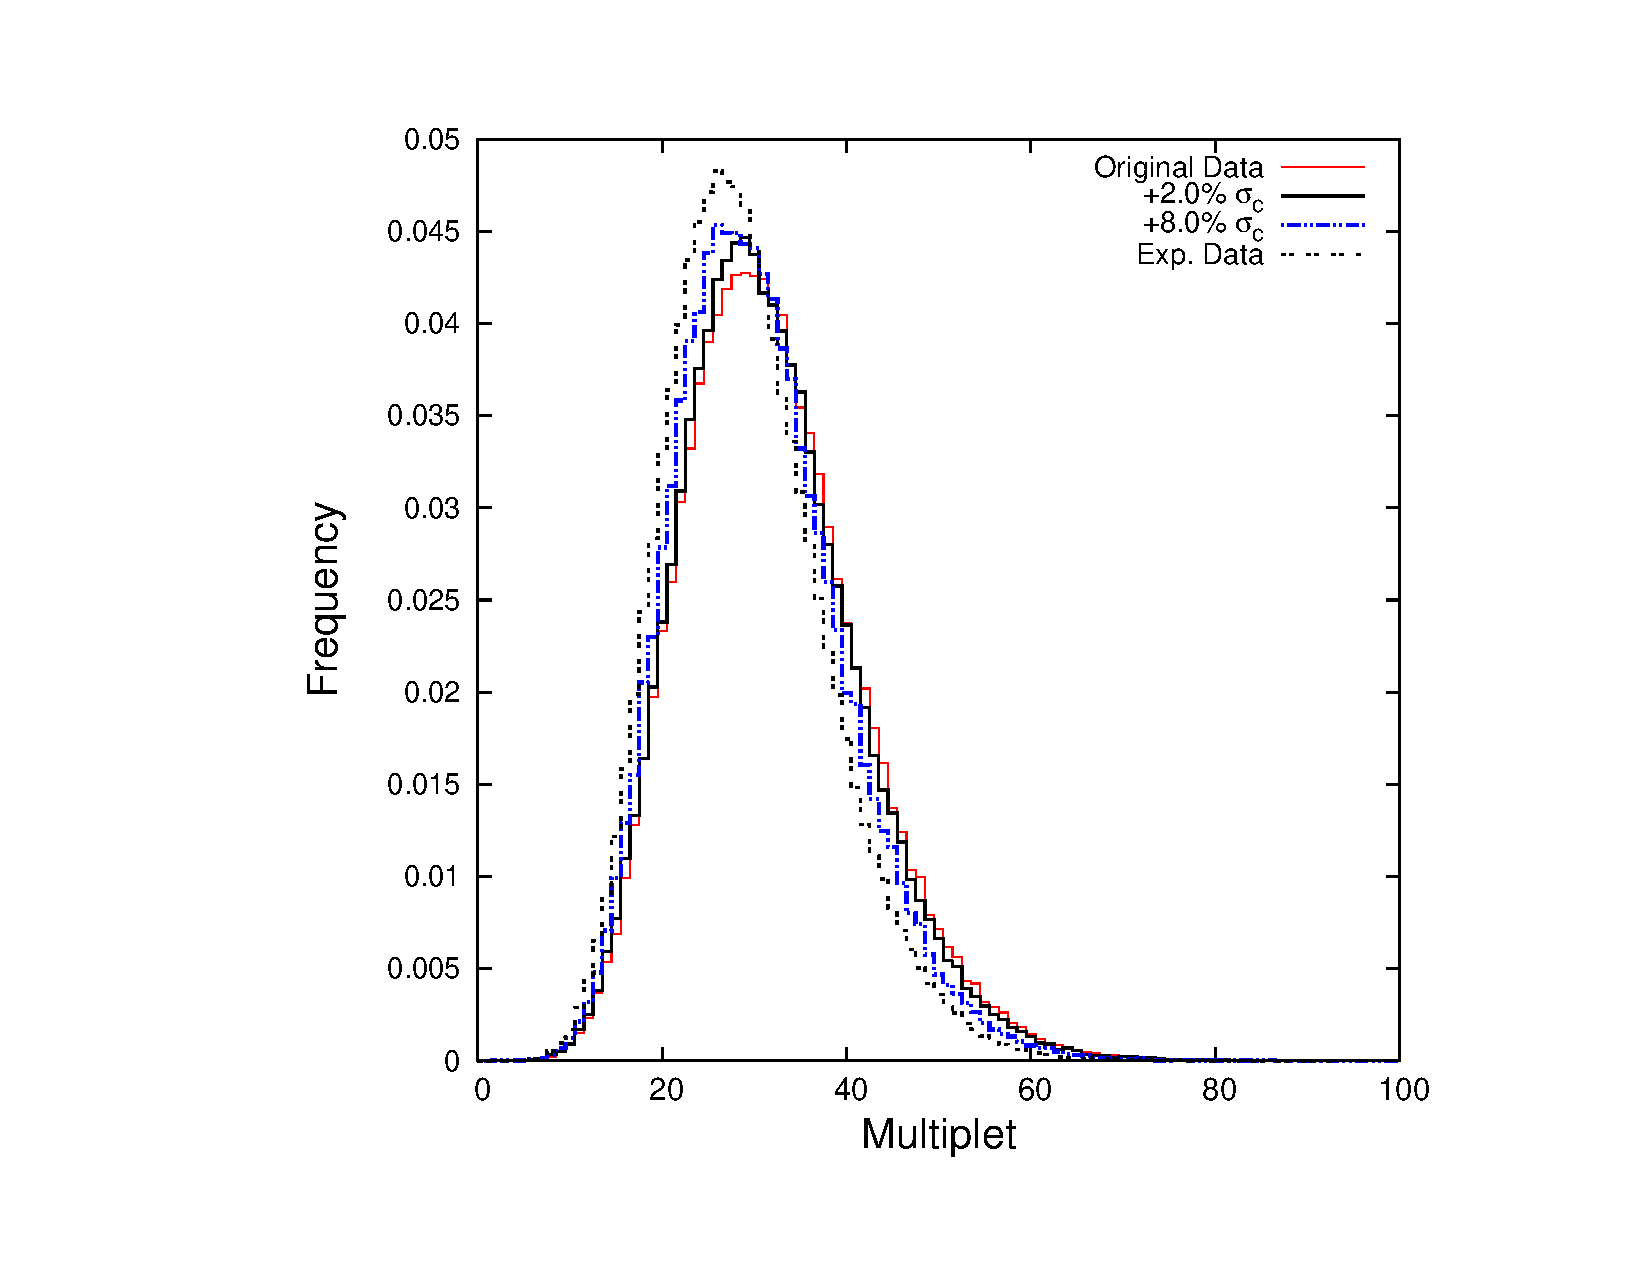
\includegraphics[trim=1.05in 0.75in 0.75in 0.75in, clip, width=1.099\textwidth]{capFigures/capture_3.pdf}
\end{minipage}	

\end{frame} 

\begin{frame}
\frametitle{Capture Cross Section}	
\begin{itemize} 
	\item Adjust \colb{total cross section} ($\sigma_t$) to compensate for change in $\sigma_c$
	\begin{equation*}
	\begin{array}{ccc}
%	\boxed{
	\boxed{\sigma'_t = \sigma_t + \epsilon_c}\hspace{0.4in} &  \epsilon_c = \alpha\,\sigma_c &\hspace{0.4in} \sigma'_c = \sigma_c + \epsilon_c%}
	\end{array}
	\end{equation*}
	\end{itemize}
	\pause
\begin{minipage}{0.49\textwidth}
\begin{table}[t!] 
	\vspace{-0.63870in} \pause
  \begin{center}
	\resizebox{0.99\textwidth}{!}{
  \begin{tabular}{|ccccc|}
    \hline Trial & {$\chi^2_{\,mult}$} &
    {$\chi^2_{\,{k}_{eff}}$} &  {$\#s(\sigma_t)$}
  &   {$\#s(\sigma_c)$} 
   \\  \hline
    \nubar -1.14\% & 130.6 & 33.66 & n/a  & n/a \\
\colg{$\mathbf{\alpha=16.0\%}$} & \colg{142.6} & \colg{1.86} & \colg{3.47} & \colg{6.90}\\
$\alpha=8.0\%$ & 237.5 & 0.51 & 1.74 &  3.45 \\ 
$\alpha=2.0\%$ & 371.2 & 0.02 & 0.43 &  0.86 \\
$\alpha=1.0\%$ & 396.4 & 0.16 & 0.22 &  0.43 \\
Original & 426.6 & 0.27 & 0 & 0  \\ \hline
  \end{tabular}}
  \end{center}
\end{table}
\end{minipage}
\begin{minipage}{0.49\textwidth}
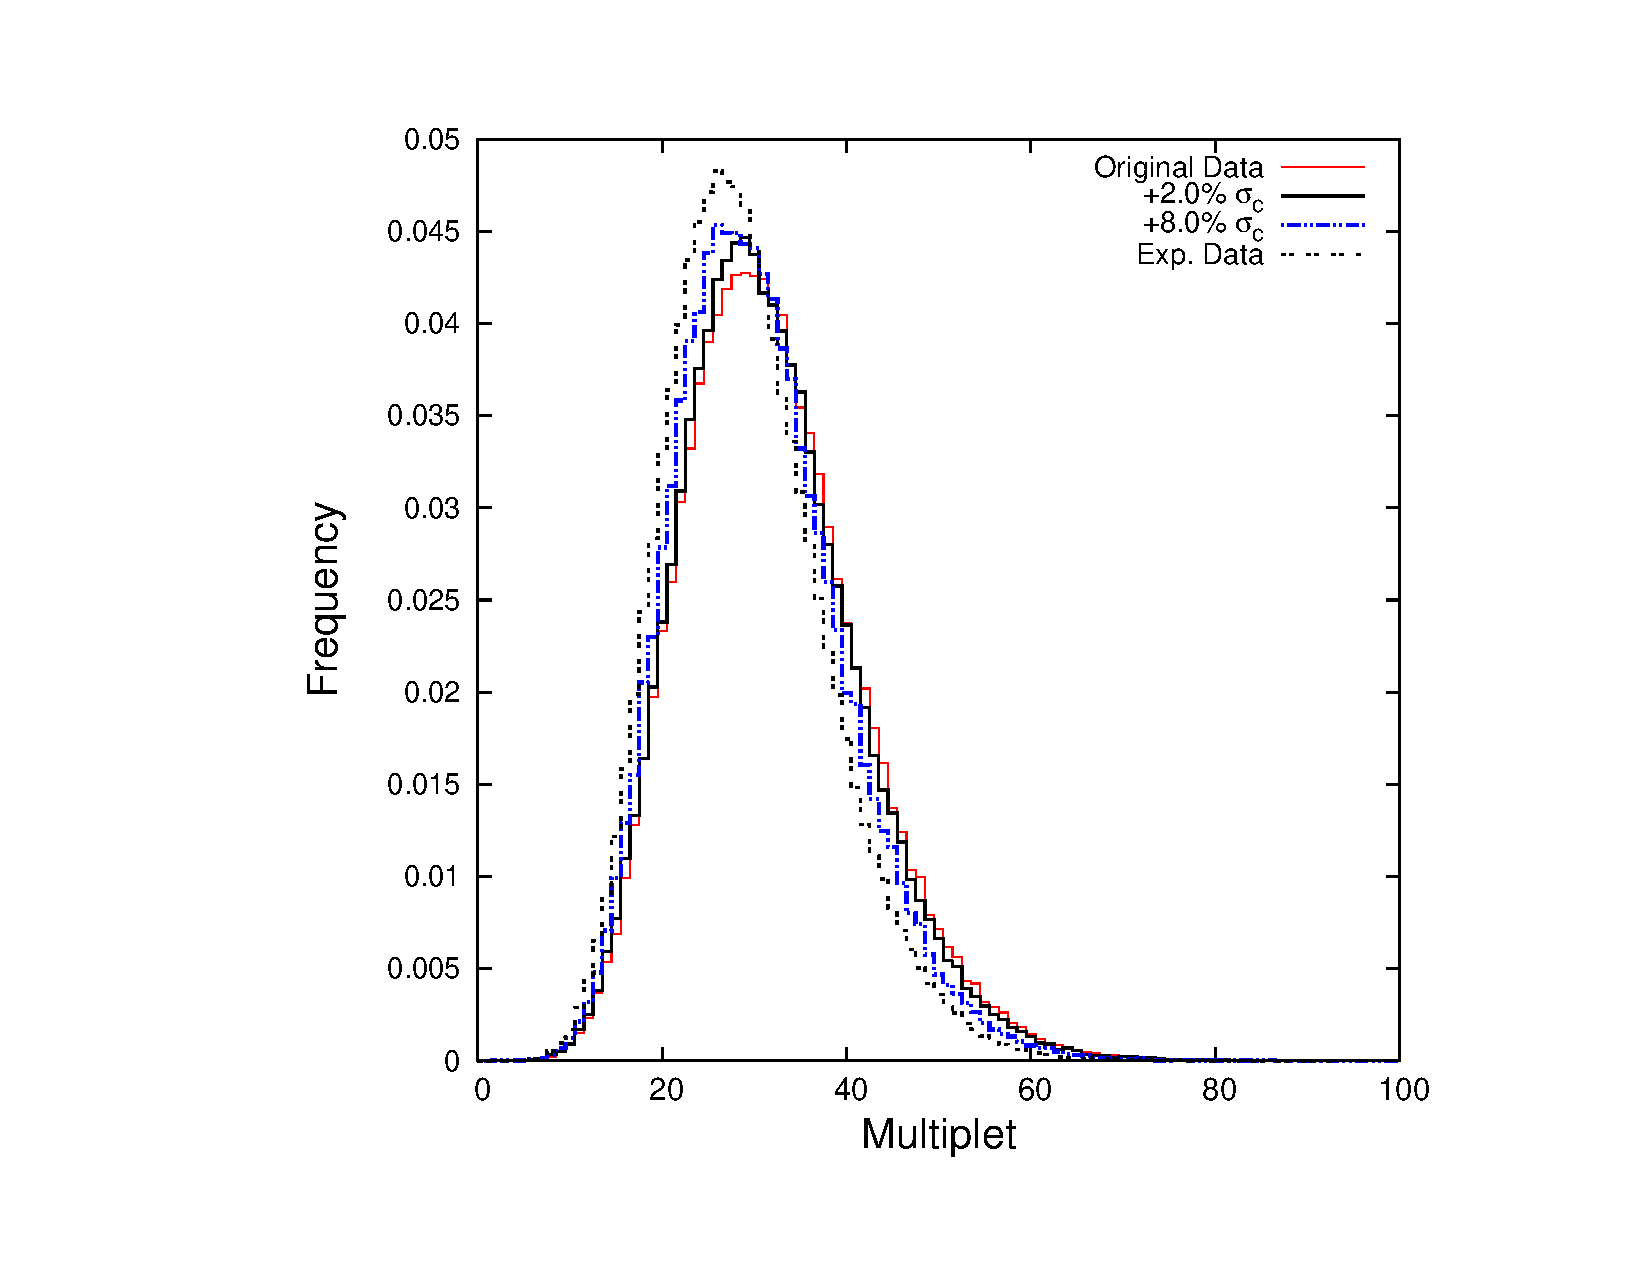
\includegraphics[trim=1.05in 0.75in 0.75in 0.75in, clip, width=1.099\textwidth]{capFigures/capture_3.pdf}
\end{minipage}	

\end{frame} 



\begin{frame}
\frametitle{Fission Cross Section}
\begin{itemize}
  \item Adjust \colb{elastic scattering} ($\sigma_s$) to compensate for change in $\sigma_f$
	\begin{equation*}
	\begin{array}{ccc}
%	\boxed{
	\boxed{\sigma'_s = \sigma_s + \epsilon_f}\hspace{0.4in} &  \epsilon_f = {\colb{-}}\alpha\,\sigma_f &\hspace{0.4in} \sigma'_f = \sigma_f \colb{-} \epsilon_f%}
	\end{array}
	\end{equation*}
	\item \colb{Only} {for} $E>1 keV$
\end{itemize} 
\pause

\begin{table}[h!] 
	\vspace{-0.1in}
  \begin{center}
	\resizebox{0.345\textwidth}{!}{
  \begin{tabular}{|ccc|}
    \hline {Trial} & {$\chi^2_{\,mult}$} &
    {$\chi^2_{\,{k}_{eff}}$}  \\ \hline
    $\alpha = 2.0$\% & 65.8 & 29.6 \\ 
    $\alpha = 1.5\%$ & 14.6 & 24.4 \\ 
    $\alpha = 1.0\%$ & 56.5 & 9.4 \\ 
    $\alpha = 0.5\%$ & 195.7 & 3.0 \\ 
   \nubar -1.14\% & 130.58 & 33.7 \\
    Original\% & 426.6 & 0.0  \\  \hline
  \end{tabular}}
  \end{center}
\end{table}

\end{frame} 

\begin{frame}
\frametitle{Future Work}
\vspace{-0.86in}
\begin{itemize}
  \item More energy-dependent \nubar trials \pause
%	\item Need covariance data for \sfiss and $\sigma_s$ \pause
	\item Energy-dependent \sfiss trials \pause
	\begin{itemize}
		\item \sfiss has \colb{400} covariance energy groups vs \colb{50} for \nubar
		\item Need constrained global optimization method
	\end{itemize}\pause



\end{itemize} 

\end{frame} 



\setcounter{framenumber}{\value{finalframe}}

